\documentclass{beamer}
\setbeamertemplate{navigation symbols}{}

\usepackage{hyperref}
\usepackage{dirtytalk}
\usepackage{emoji}
\usepackage[utf8]{inputenc}
\usepackage[
  english,
  spanish,
  es-tabla,
  es-nodecimaldot
]{babel}
\selectlanguage{spanish}
\usepackage{minted}
\setminted[python]{frame=single,autogobble,linenos,numbersep=4pt}

\usetheme{Rochester}
\definecolor{pinky}{rgb}{0.9098, 0.2627, 0.4431}
\usecolortheme[named=pinky]{structure}

\title{{\Huge\emoji{technologist-light-skin-tone}}\\¡Comenzando con Python!}
\author{Sergio García Prado}
\date{\today}

\begin{document}

    \begin{frame}
        \titlepage
    \end{frame}

    \begin{frame}{Sobre mi}
      \noindent
      \begin{minipage}{.24\textwidth}
          \begin{figure}
            \centering
            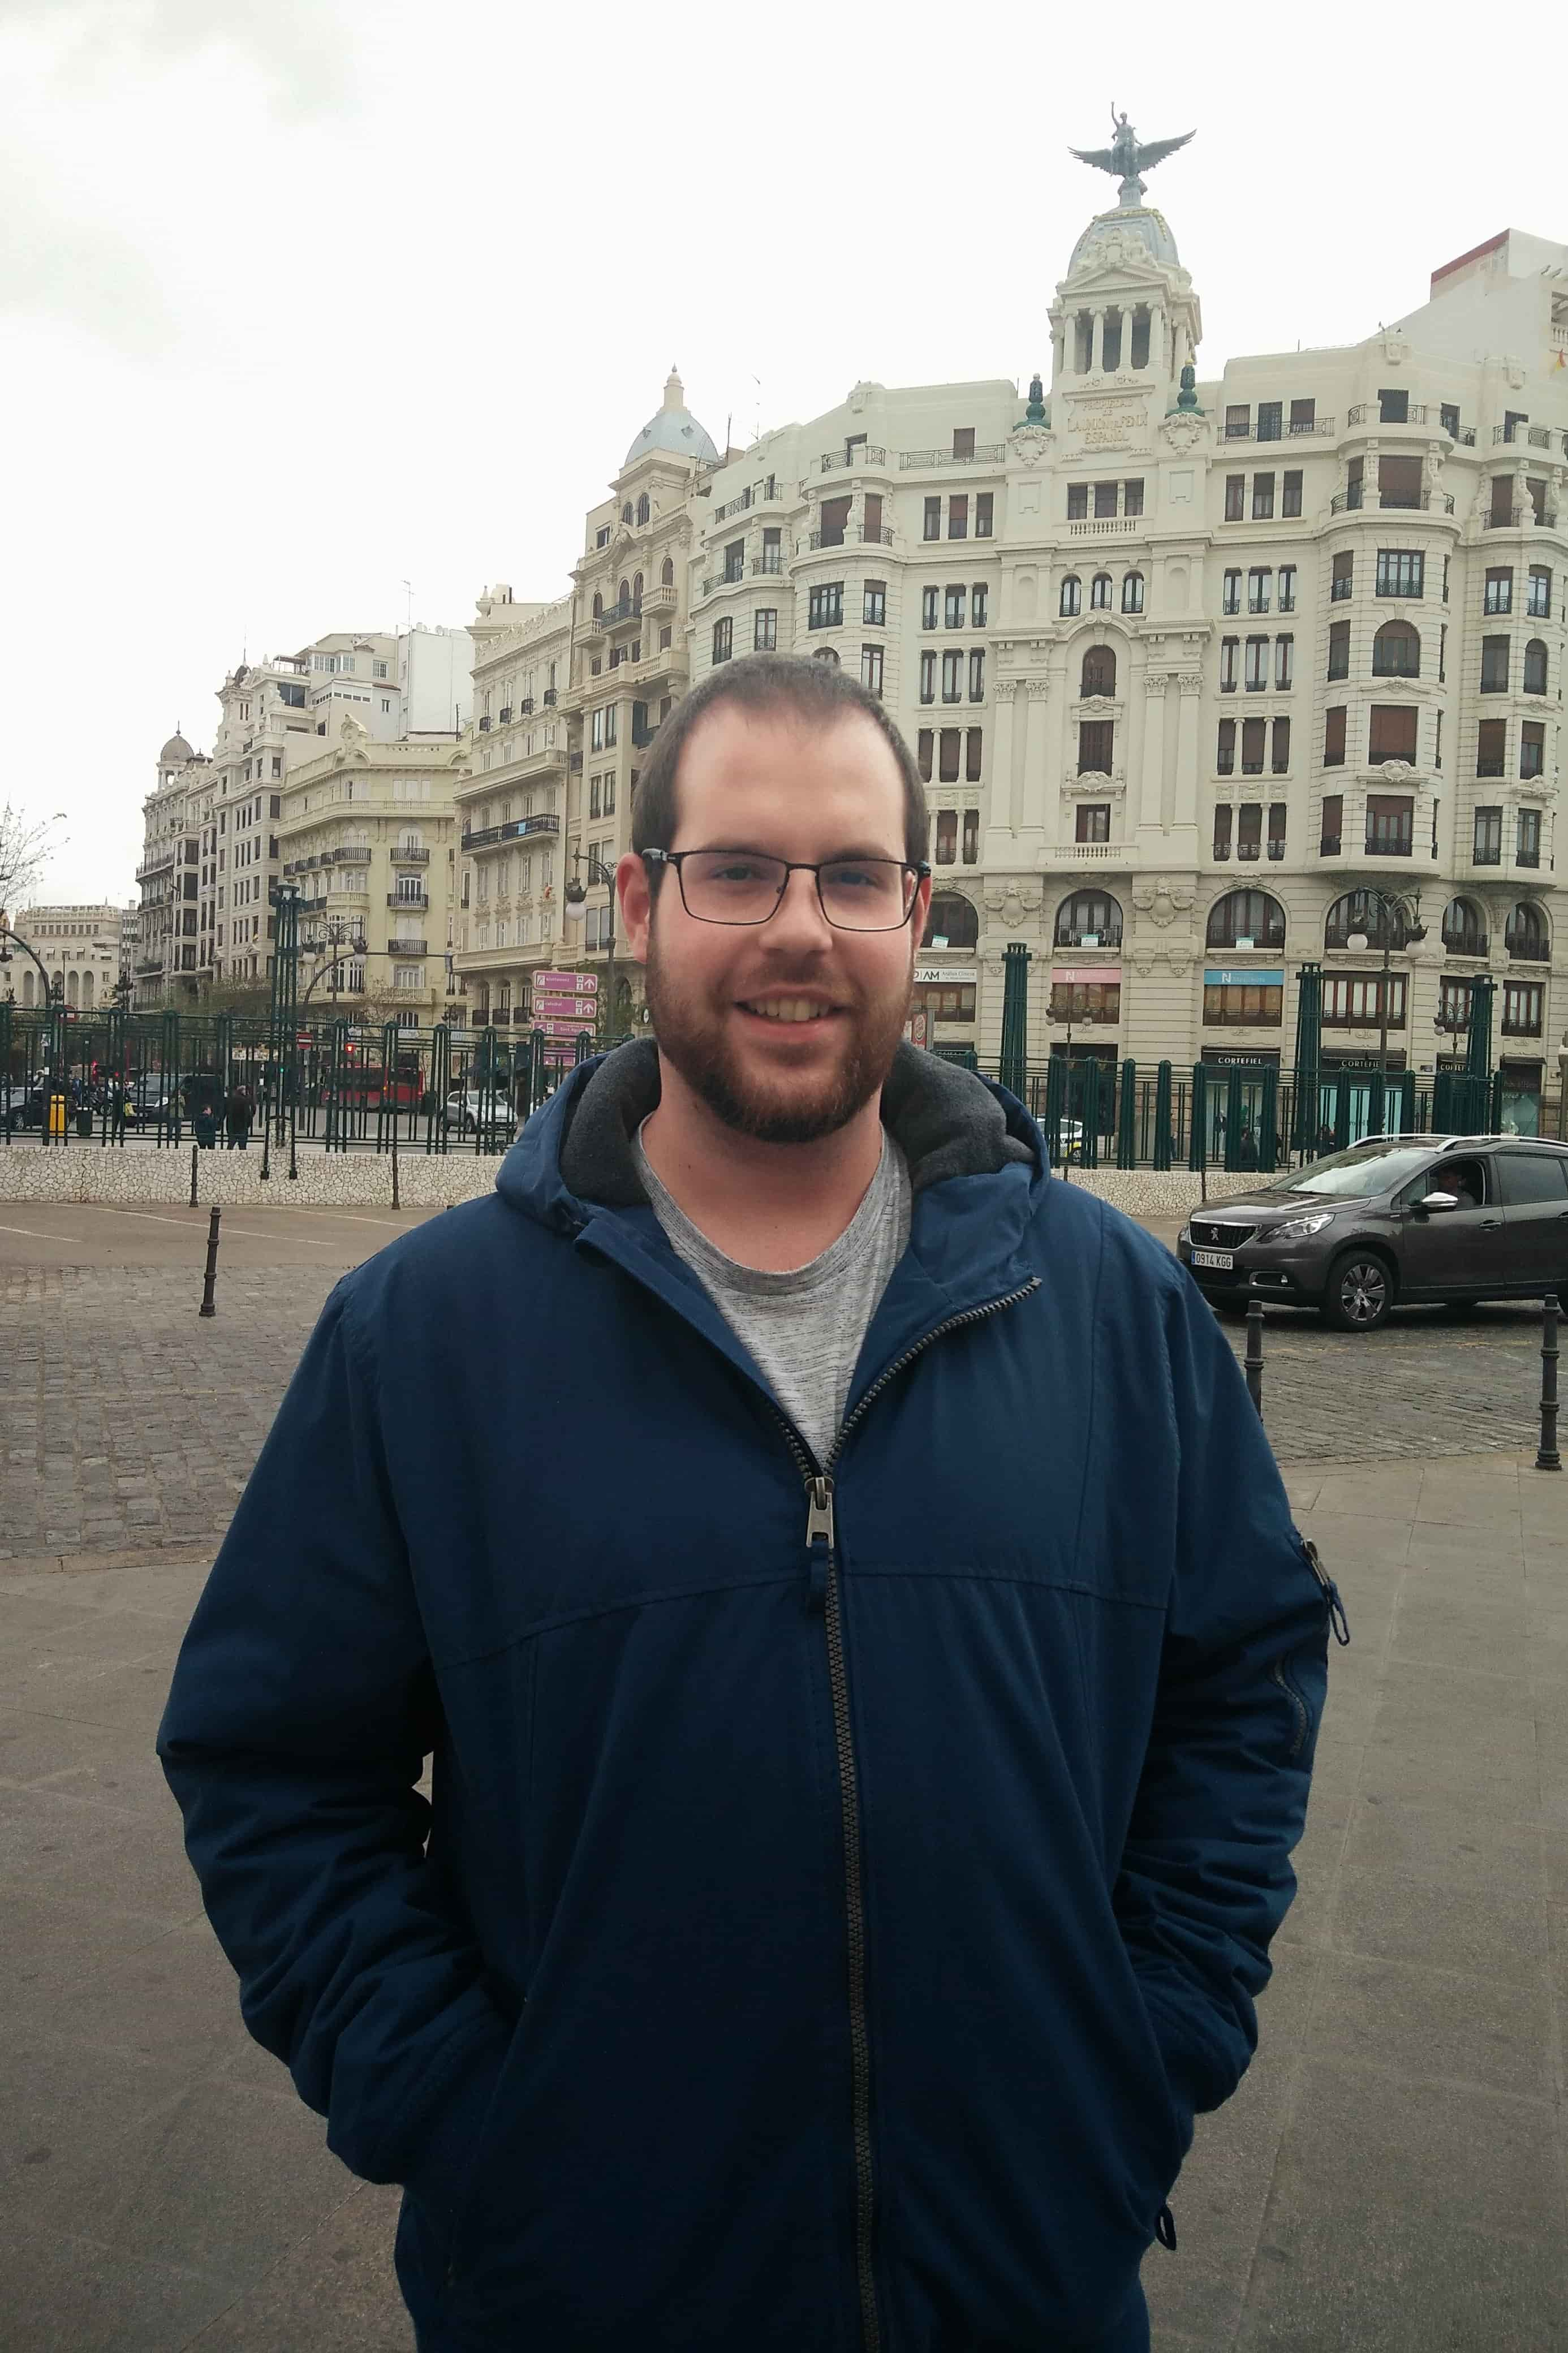
\includegraphics[width=\textwidth]{images/photo}
          \end{figure}
      \end{minipage}
      \begin{minipage}{.74\textwidth}
          \begin{itemize}
            \item ¡Hola! Soy Sergio García Prado
            \item Estudios:
            \begin{itemize}
              \item [\emoji{desktop-computer}] Graduado en Ingeniería Informática
              \item [\emoji{chart-increasing}] Graduado en Estadística
            \end{itemize}
            \item Experiencia Laboral:
            \begin{itemize}
              \item [\emoji{rocket}] Software Engineer/ Data Scientist en Unlimiteck
            \end{itemize}
            \item Sígueme:
                \begin{itemize}
                    \item Mail: \href{mailto:sergio@garcipardes.me}{sergio@garcipardes.me}
                    \item Website: \href{http://garciparedes.me}{garciparedes.me}
                    \item GitHub: \href{http://github.com/garciparedes}{@garciparedes}
                    \item LinkedIn: \href{https://www.linkedin.com/in/garciparedes/}{Sergio García Prado}
                \end{itemize}
          \end{itemize}
      \end{minipage}
    \end{frame}

    \begin{frame}{¿En qué consiste la programación?}
      \noindent
      \begin{minipage}{.69\textwidth}
          \say{La programación es el proceso utilizado para idear y ordenar las acciones necesarias para realizar un proyecto, preparar ciertas máquinas o aparatos para que empiecen a funcionar en el momento y en la forma deseados o elaborar programas para su empleo en computadoras}
          \rightline{{\rm ---  R.A.E. (2014)}}
      \end{minipage}
      \begin{minipage}{.29\textwidth}
          \begin{center}
            \fontsize{40}{50}
              \emoji{computer}
          \end{center}
      \end{minipage}
    \end{frame}

    \begin{frame}{Similitud con recetas de cocina}
        \noindent
        \begin{minipage}{.29\textwidth}
          \begin{center}
            \fontsize{40}{50}
              \emoji{cake}
          \end{center}
        \end{minipage}
        \begin{minipage}{.69\textwidth}
            \begin{itemize}
                \item La idea de programar sobre un ordenador no es muy diferente de tareas como la de seguir una receta.
                \item Receta de Bizcocho:
                \begin{enumerate}
                    \item Mezclar ingredientes secos.
                    \item Mezclar ingredientes húmedos.
                    \item Combinar todos los ingredientes.
                    \item Encender el horno.
                    \item Amasar hasta conseguir una masa homogénea.
                    \item Hornear durante 30 minutos.
                    \item Dejar reposar.
                \end{enumerate}
            \end{itemize}
        \end{minipage}
    \end{frame}

    \begin{frame}{Pensamiento jerárquico}
        \begin{itemize}
          \item El mundo de la programación se cimienta sobre la construcción de abstracciones sobre conceptos básicos, que de manera conjunta forman una base de conocimiento más rica.
          \item Ejemplo:
          \begin{itemize}
            \item Hacer bizcocho
            \item Mezclar ingredientes secos, ...
            \item Mezclar harina, azúcar, levadura, ...
            \item Introducir harina en el recipiente, introducir azúcar en el recipiente, ...
            \item Abrir paquete de harina, calcular cantidad de harina, ...
            \item ...
          \end{itemize}
        \end{itemize}
    \end{frame}

    \begin{frame}{¡Hola, Mundo!}
      \noindent
      \begin{minipage}{.69\textwidth}
        \begin{itemize}
          \item El término \emph{Hello, World} consiste en la ejemplificación sobre las sentencias necesarias para un lenguaje de programación determinado, de tal manera que este imprima por consola el texto \texttt{Hello, World!}.
          \item Hola mundo en \emph{Python}: \mintinline{python}{print("Hello, World!")}
        \end{itemize}
      \end{minipage}
      \begin{minipage}{.29\textwidth}
          \begin{center}
            \fontsize{40}{50}
              \emoji{man-raising-hand-light-skin-tone}\emoji{earth-africa}
          \end{center}
      \end{minipage}
    \end{frame}

    \begin{frame}{¿Por qué Python?}
        \noindent
        \begin{minipage}{.29\textwidth}
            \begin{center}
              \fontsize{40}{50}
                \emoji{snake}
            \end{center}
        \end{minipage}
        \begin{minipage}{.69\textwidth}
          \begin{itemize}
            \item \emph{Python} es un lenguaje de programación interpretado cuya filosofía hace hincapié en la \emph{legibilidad de su código}.​ bu
            \item En los últimos años ha sufrido un crecimiento exponencial, entre otros, por el ecosistema de tan heterogéneo que se ha ido construyendo a su alrededor: \emph{Data Science}, \emph{Web Development}, \emph{Embedded Systems}, etc.
          \end{itemize}
        \end{minipage}
    \end{frame}

    \begin{frame}{Conceptos básicos: Variables}
        \begin{itemize}
            \item El concepto más básico e importante para aprender a programar es el de \emph{variable}.
            \item Una variable consiste en un identificador a partir del cual se puede acceder a la información que este tiene asignada.
            \item En \emph{Python}, se puede asignar información a una variable de la siguiente forma: \mintinline{python}{variable = expression}
            \begin{itemize}
                \item \emph{variable} representa el identificador.
                \item \emph{expression} representa la información que contiene la variable.
            \end{itemize}
            \item Ejemplos:
            \begin{itemize}
                \item \mintinline{python}{x = 3}
                \item \mintinline{python}{y = "Hello"}
                \item \mintinline{python}{x = y}
                \item \mintinline{python}{z = [x, y]}
            \end{itemize}
        \end{itemize}
    \end{frame}

    \begin{frame}{Conceptos básicos: Tipos de Datos}
        \begin{itemize}
            \item Las variables tienen asociado un determinado tipo.
            \item En \emph{Python} este puede cambiar a lo largo de la ejecución (\emph{tipado dinámico}).
            \item Existe un valor especial para indicar que la variable no contiene ningún valor (y por tanto tampoco tipo) denominado \mintinline{python}{None}.
            \item Algunos de los tipos más populares son los siguientes:
            \begin{itemize}
                \item Texto (\mintinline{python}{str}): \mintinline{python}{x = "Hello!"}
                \item Enteros (\mintinline{python}{int}): \mintinline{python}{x = 56}
                \item Decimales (\mintinline{python}{float}): \mintinline{python}{x = -3.14}
                \item Booleanos (\mintinline{python}{bool}): \mintinline{python}{x = True}
                \item Listas (\mintinline{python}{list}): \mintinline{python}{x = [1, None, 2, "Hello", False]}
                \item Diccionarios (\mintinline{python}{dict}): \mintinline{python}{x = {"a": 1, "b": 3, None: False}}
            \end{itemize}
        \end{itemize}
    \end{frame}

    \begin{frame}{Conceptos básicos: Operaciones Básicas}
        \begin{itemize}
            \item La siguiente característica de las variables es que estas poseen operaciones que modifican su estado (de manera individual o conjunta).
            \item Dichas operaciones dependen del tipo de información que estas contengan.
            \item Algunos ejemplos:
            \begin{itemize}
                \item Suma (\mintinline{python}{int, float, str, list}): \mintinline{python}{z = x + y}
                \item Multiplicación (\mintinline{python}{int, float, str, list}): \mintinline{python}{z = x * y}
                \item Igualdad (\mintinline{python}{object}): \mintinline{python}{z = (x == y)}
                \item Negación (\mintinline{python}{bool}): \mintinline{python}{y = not x}
                \item Adicción (\mintinline{python}{list}): \mintinline{python}{x.append(y)}
                \item Lectura (\mintinline{python}{dict}): \mintinline{python}{x["a"]}
            \end{itemize}
        \end{itemize}
    \end{frame}

    \begin{frame}[fragile]{Conceptos básicos: Condicionales}
        \begin{itemize}
          \item Además de las operaciones entre variables, existen situaciones en que es necesario tomar decisiones diferentes dependiendo de una determinada condición, lo cual se traduce en la ejecución de diferentes sentencias de código.
          \item Para ello, se utilizan sentencias \mintinline{python}{if} - \mintinline{python}{elif} - \mintinline{python}{else} de la siguiente forma:

          \begin{figure}
              \begin{minipage}[c]{0.5\textwidth}
                  \begin{minted}[fontsize=\tiny]{python}
                      if condition1:
                        ...
                      elif condition2:
                        ...
                      ...
                      else:
                        ...
                  \end{minted}
              \end{minipage}
          \end{figure}
          \item Ejemplo:
          \begin{figure}
              \begin{minipage}[c]{0.5\textwidth}
                  \begin{minted}[fontsize=\tiny]{python}
                      if x < 3:
                          print("x less than 3")
                      elif x == 3:
                          print("x equal to 3")
                      else:
                          print("x greater than 3")
                  \end{minted}
              \end{minipage}
          \end{figure}
        \end{itemize}
    \end{frame}


    \begin{frame}[fragile]{Conceptos básicos: Bucles}
        \begin{itemize}
          \item Cuando se programa, es común repetir una determinada acción durante un número determinado de veces, ya sea debido a una condición dada o para procesar una colección de elementos.
          \item En \emph{Python}, esto se lleva a cabo a través de sentencias \mintinline{python}{while} o \mintinline{python}{for}. Además, existen palabras clave para modificar su comportamiento como \mintinline{python}{break} o \mintinline{python}{continue}

          \begin{figure}
              \begin{minipage}[c]{0.5\textwidth}
                  \begin{minted}[fontsize=\tiny]{python}
                      while condition:
                        ...

                      for item in iterable:
                        ...
                  \end{minted}
              \end{minipage}
          \end{figure}
          \item Ejemplo:
          \begin{figure}
              \begin{minipage}[c]{0.5\textwidth}
                  \begin{minted}[fontsize=\tiny]{python}
                  x = 1
                  while x < 56:
                    x *= 2

                  for item in ["hello", "bye"]:
                      print(item)
                  \end{minted}
              \end{minipage}
          \end{figure}
        \end{itemize}
    \end{frame}

    \begin{frame}{Caso Práctico: Recordatorios (I)}
        \noindent
        \begin{minipage}{.69\textwidth}
          \begin{itemize}
            \item Para ejemplificar cómo usar \emph{Python} así como sus intrucciones básicas se propone construir una aplicación básica de recordatorios.
            \item Por motivos de simplicidad, por el momento la aplicación permitirá únicamente las siguientes historias de usuario:
              \begin{itemize}
                \item Añadir nuevos recordatorios.
                \item Listar recordatorios existentes.
              \end{itemize}
          \end{itemize}
        \end{minipage}
        \begin{minipage}{.29\textwidth}
            \begin{center}
              \fontsize{40}{50}
                \emoji{memo}
            \end{center}
        \end{minipage}
    \end{frame}

    \begin{frame}[fragile]{Caso Práctico: Recordatorios (II)}
        \begin{itemize}
          \item ¿Cómo leer los recordatorios?
            \begin{figure}
              \begin{minipage}[c]{0.7\textwidth}
                  \begin{minted}[fontsize=\tiny]{python}
                      message = input("What to reminder? --> ")
                      seconds = int(input("How many seconds? --> "))
                      reminder = [False, seconds, message]
                      print(f"Created a reminder: {reminder}")
                  \end{minted}
                \end{minipage}
            \end{figure}
          \item ¿Dónde almacenar los recordatorios?
          \begin{figure}
              \begin{minipage}[c]{0.7\textwidth}
                  \begin{minted}[fontsize=\tiny]{python}
                      reminders = list()
                      reminders.append(reminder)
                  \end{minted}
              \end{minipage}
          \end{figure}
        \end{itemize}
    \end{frame}

    \begin{frame}[fragile]{Caso Práctico: Recordatorios (III)}
        \begin{itemize}
          \item ¿Cómo mostrar los resultados?
          \begin{figure}
              \begin{minipage}[c]{0.7\textwidth}
                  \begin{minted}[fontsize=\tiny]{python}
                        print("Remainders:")
                        print("\tCompleted\tRemaining\tMessage")
                        for reminder in reminders:
                            print(f"\t{reminder[0]:>8}\t{reminder[1]:>9}\t{reminder[2]}")
                  \end{minted}
              \end{minipage}
          \end{figure}
          \item ¿Cómo controlar el modo?
          \begin{figure}
              \begin{minipage}[c]{0.7\textwidth}
                  \begin{minted}[fontsize=\tiny]{python}
                      while True:
                          command = input()
                          if command == "q":
                              break
                          elif command == "a":
                              ...
                          elif command == "s":
                              ...
                  \end{minted}
              \end{minipage}
          \end{figure}
        \end{itemize}
    \end{frame}

    \begin{frame}[fragile]{Caso Práctico: Recordatorios (III)}
      \begin{itemize}
        \item La apliación completa tiene la siguiente forma:
        \begin{figure}
            \begin{minipage}[c]{\textwidth}
                \begin{minted}[fontsize=\tiny]{python}
                reminders = list()
                while True:
                    command = input()
                    for reminder in reminders:
                        if reminder[1] - time() >= 0:
                            break
                        reminder[0] = True
                    reminders.sort()
                    if command == "q":
                        break
                    elif command == "a":
                        message = input("What to reminder? --> ")
                        seconds = round(time()) + int(input("How many seconds? --> "))
                        reminder = [False, seconds, message]
                        reminders.append(reminder)
                        print(f"Created a reminder: {reminder}")
                        print()
                    elif command == "s":
                        print("Remainders:")
                        print("\tCompleted\tRemaining\tMessage")
                        for reminder in reminders:
                            print(f"\t{reminder[0]}\t\t{reminder[1] - round(time()):>9}\t{reminder[2]}")
                        print()

                    sleep(0.5)
                \end{minted}
            \end{minipage}
        \end{figure}
      \end{itemize}
    \end{frame}

    \begin{frame}
        \begin{center}
            \Huge
            ¿Preguntas?
        \end{center}
    \end{frame}
\end{document}
